%!TEX root = ../../report.tex
\chapter{Experimental setup} % (fold)
\label{cha:experiments}
During the simulation chapter \ref{cha:simulation}, some tools were created along with the robot in order to carry out specific experiments.
In that case the robot was restricted to the movement in one plane and this was achieved with a rotational holder with an arm long enough to consider the dynamics associated with the turn negligible.
This experimental setup was inspired by the already used in the Dacbot \cite{dacbot1} in the LPZ Robots simulator \cite{lpzrobots}.

The rotational holder was built for the real Dacbot robot due to its small size made it feasible.
However, the dimensions of RuBi made not possible to create the same kind of test bench.
Another one then was created by making use of an existing treadmill modified to control the speed by an associated computer.
Thus, an structure that could allow the same restrictions as in the simulation over the treadmill was designed and implemented.

It consists of a set of 3D printed parts and standard components, such as Bosch profiles and carbon fiber tubes, that allow two degrees of freedom (DoF).
These are: (1) a vertical displacement that let the robot the necessary freedom for jumping and (2) a rotation over an axis that allows the robot to adapt its inclination when running or walking. 
This last one can be locked to a specific inclination though. In the figures \ref{fig:photo_structure} and \ref{fig:legs_structure}, a render and a photo of the real structure are presented.

\begin{figure}[ht!]
    \centering
    \begin{subfigure}[b]{0.49\textwidth}
        \includegraphics[width=\textwidth]{figures/photo_structure.jpg}
        \caption{RuBi in the test bench assembled}
        \label{fig:photo_structure}
    \end{subfigure}
    \begin{subfigure}[b]{0.49\textwidth}
        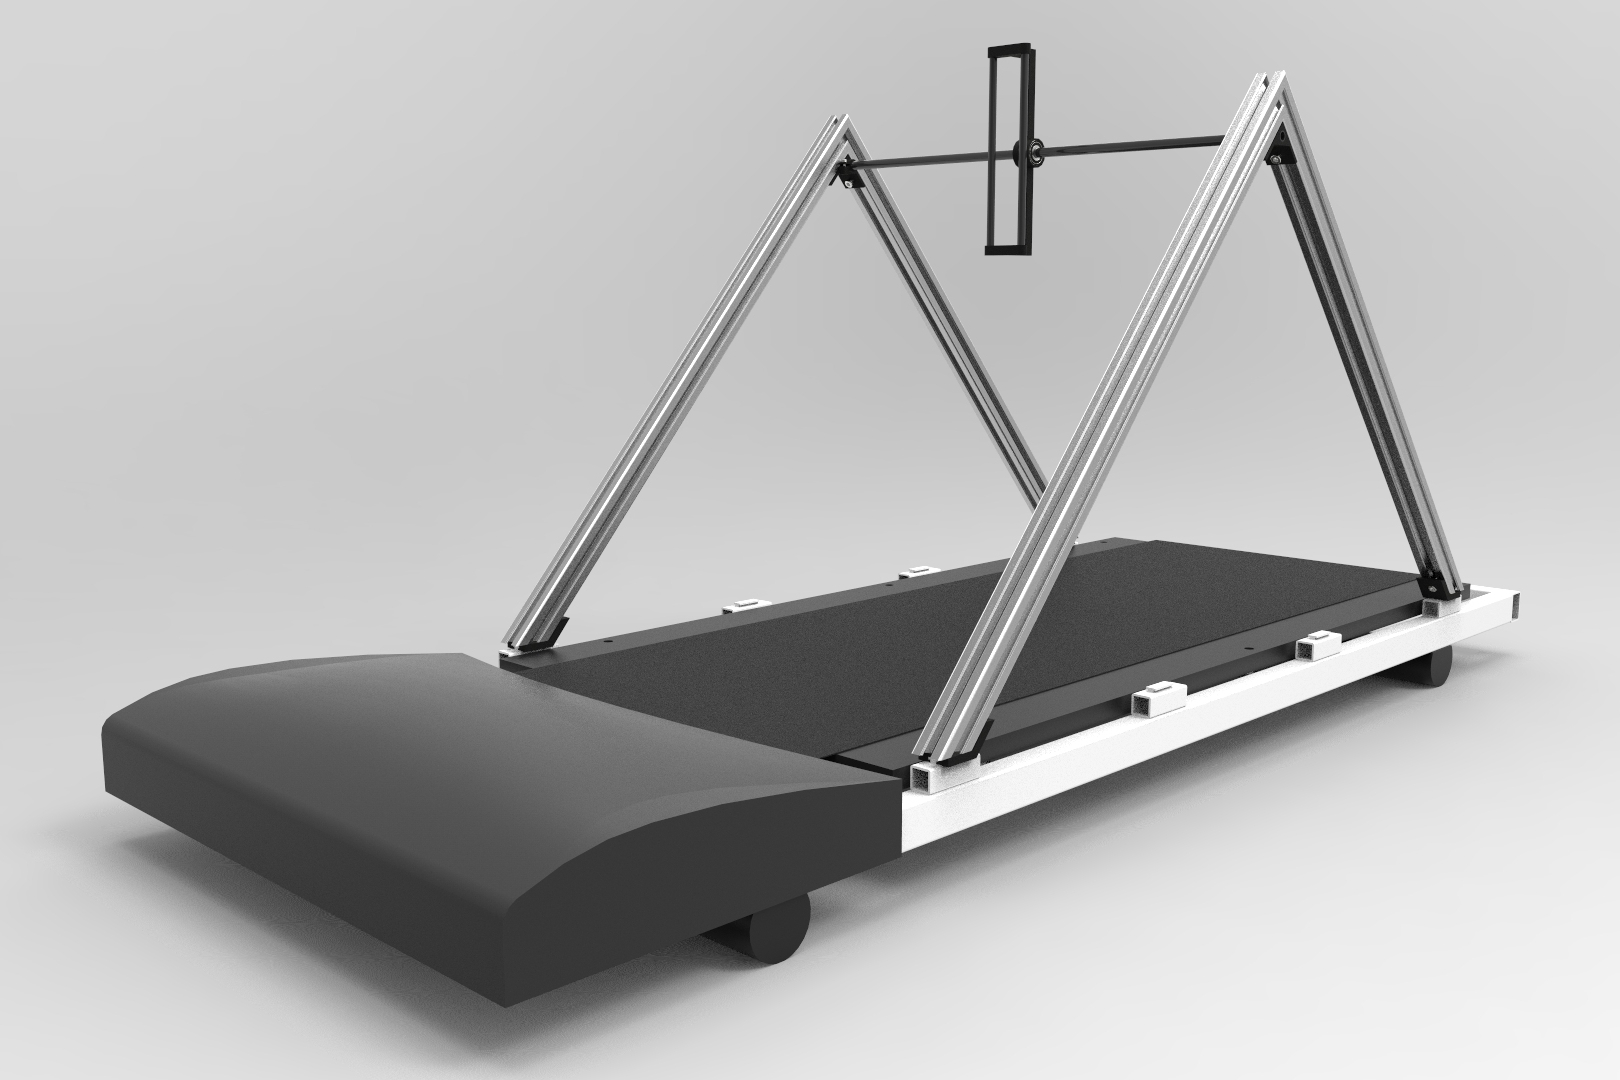
\includegraphics[width=\textwidth]{figures/legs_structure.jpg}
        \caption{Test bench for RuBi rendering}
        \label{fig:legs_structure}
    \end{subfigure}
\end{figure}  

\todo{Jump platform devise and experimentation}
%Virtual compliant leg model here --> used for experimentation and testing of the theoretical frame introduced in \ref{sec_springs}.

\begin{figure}[ht!]
    \centering
    \begin{subfigure}[b]{0.25\textwidth}
        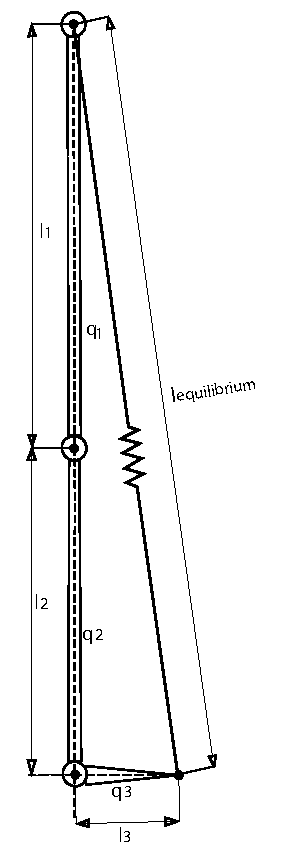
\includegraphics[width=\textwidth]{figures/spring_model_equilibrium.pdf}
        \caption{RuBi in the test bench assembled}
        \label{fig:virtual_spring1}
    \end{subfigure}
    \begin{subfigure}[b]{0.25\textwidth}
        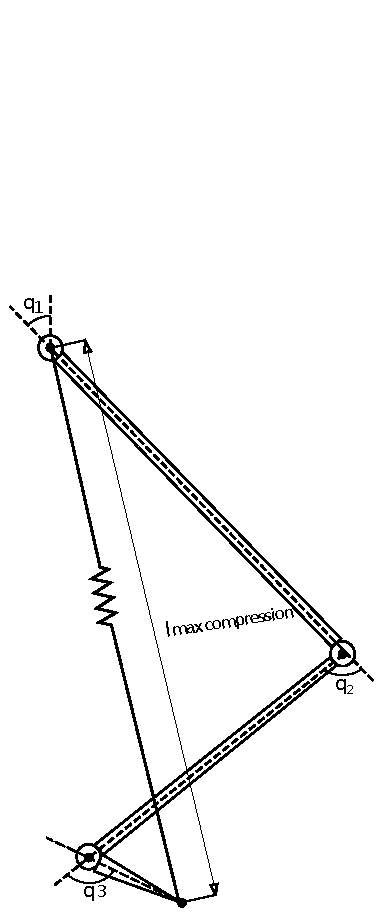
\includegraphics[width=\textwidth]{figures/spring_model_max_compressed.pdf}
        \caption{Test bench for RuBi rendering}
        \label{fig:virtual_spring2}
    \end{subfigure}
    \begin{subfigure}[b]{0.25\textwidth}
        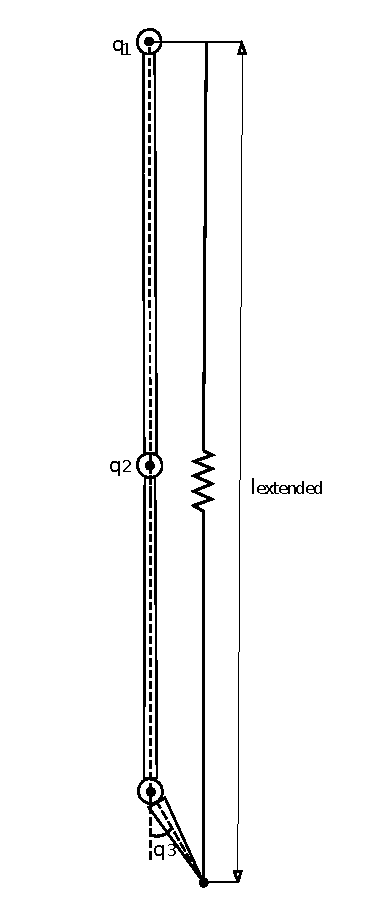
\includegraphics[width=\textwidth]{figures//spring_model_max_extended.pdf}
        \caption{Test bench for RuBi rendering}
        \label{fig:virtual_spring3}
    \end{subfigure}
\end{figure}  

% chapter experiments (end)